% ******************************************************** %
%              TEMPLATE DE INFORME ORGA2 v0.1              %
% ******************************************************** %
% ******************************************************** %
%                                                          %
% ALGUNOS PAQUETES REQUERIDOS (EN UBUNTU):                 %
% ========================================
%                                                          %
% texlive-latex-base                                       %
% texlive-latex-recommended                                %
% texlive-fonts-recommended                                %
% texlive-latex-extra?                                     %
% texlive-lang-spanish (en ubuntu 13.10)                   %
% ******************************************************** %


\documentclass[a4paper]{article}
\usepackage[spanish]{babel}
\usepackage[utf8]{inputenc}
\usepackage{charter}   % tipografia
\usepackage{graphicx}
\usepackage{float}
%\usepackage{makeidx}
\usepackage{paralist} %itemize inline
\usepackage[T1]{fontenc}

%\usepackage{float}
%\usepackage{amsmath, amsthm, amssymb}
%\usepackage{amsfonts}
%\usepackage{sectsty}
%\usepackage{charter}
%\usepackage{wrapfig}
%\usepackage{listings}
%\lstset{language=C}

% \setcounter{secnumdepth}{2}
\usepackage{underscore}
\usepackage{caratula}
\usepackage{url}


% ********************************************************* %
% ~~~~~~~~              Code snippets             ~~~~~~~~~ %
% ********************************************************* %

\usepackage{color} % para snipets de codigo coloreados
\usepackage{fancybox}  % para el sbox de los snipets de codigo

\definecolor{litegrey}{gray}{0.94}

\newenvironment{codesnippet}{%
	\begin{Sbox}\begin{minipage}{\textwidth}\sffamily\small}%
	{\end{minipage}\end{Sbox}%
		\begin{center}%
		\vspace{-0.4cm}\colorbox{litegrey}{\TheSbox}\end{center}\vspace{0.3cm}}



% ********************************************************* %
% ~~~~~~~~         Formato de las páginas         ~~~~~~~~~ %
% ********************************************************* %

\usepackage{fancyhdr}
\pagestyle{fancy}

%\renewcommand{\chaptermark}[1]{\markboth{#1}{}}
\renewcommand{\sectionmark}[1]{\markright{\thesection\ - #1}}

\fancyhf{}

\fancyhead[LO]{Sección \rightmark} % \thesection\ 
\fancyfoot[LO]{\small{Martin Amigo, Santiago Festini}}
\fancyfoot[RO]{\thepage}
\renewcommand{\headrulewidth}{0.5pt}
\renewcommand{\footrulewidth}{0.5pt}
\setlength{\hoffset}{-0.8in}
\setlength{\textwidth}{16cm}
%\setlength{\hoffset}{-1.1cm}
%\setlength{\textwidth}{16cm}
\setlength{\headsep}{0.5cm}
\setlength{\textheight}{25cm}
\setlength{\voffset}{-0.7in}
\setlength{\headwidth}{\textwidth}
\setlength{\headheight}{13.1pt}

\renewcommand{\baselinestretch}{1.1}  % line spacing

% ******************************************************** %


\begin{document}


\thispagestyle{empty}
\materia{Algoritmos y Estructuras de Datos III}
\submateria{Primer Cuatrimestre de 2019}
\titulo{Trabajo Práctico I}
\subtitulo{"The Knapsack Problem"}
\integrante{Amigo Martín}{362/17}{martinamigo@protonmail.com.}
\integrante{Festini Santiago}{311/17}{festini.santiago21@gmail.com}


\maketitle
\newpage

\thispagestyle{empty}
\vfill
\begin{center}
    
\includegraphics[scale=0.4]{LogoGloppiYa.png}

  \end{center}


\thispagestyle{empty}
\vspace{3cm}
\tableofcontents
\newpage


%\normalsize
\newpage

\section{Introducción}

Se nos fue propuesto el siguiente problema como inicio de una serie de mejoras a la App "Gloppi Ya!". La misma se encarga de gestionar pedidos a cadenas de supermercados, mediante \textit{compradores} que arman y pagan los pedidos, y \textit{enviadores} que los llevan a destino. El problema propuesto consiste en optimizar la asignación de los pedidos a les compradores de forma que el beneficio obtenido sea máximo. 


El modelo que se escogió para resolver el problema es el Problema de las Mochilas Múltiples o Multiple Knapsack Problem  en inglés, que busca asignar de manera óptima un conjunto de ítems a un conjunto de compradores. Sin embargo, nos pareció conveniente simplificar el mismo al caso de un solo comprador, modelándolo así con el Problema de la Mochila o Knapsack problem. 

Más en detalle, el problema es el siguiente: se nos son dadas la capacidad $W$ de la mochila del comprador y una lista $S$ de pedidos, representados como pares $<w_i, p_i>$, donde $w_i$ es el tamaño y $p_i$ el beneficio del pedido correspondiente. Nuestro objetivo es encontrar la mejor asignación posible, es decir, el subconjunto de pedidos que maximice la suma de sus beneficios $p_i$, y cuya suma de tamaños $w_i$ no sobrepase la capacidad $W$ de la mochila. 

%NO OBSTANTE%

%poner ejemplos del problema y un grafiquito%

A continuación (Tabla 1.a) se provee un ejemplo de entrada y su salida esperada. La Figura 1.a ilustra el mismo.

\begin{center}
\begin{tabular}{ |c|c| } 
 \hline
 \textbf{Entrada de ejemplo} & \textbf{Salida esperada}  \\ 
 \hline
 5  \quad 25  & 29  \\ 
 10 \quad  5 &   \\ 
 15  \quad 4 & \\
 5  \quad 13 & \\
 10 \quad  8 & \\
 5 \quad  8 & \\
 \hline
\end{tabular}

\bigskip


\caption{Tabla 1.a}
\end{center}

  \begin{center}
    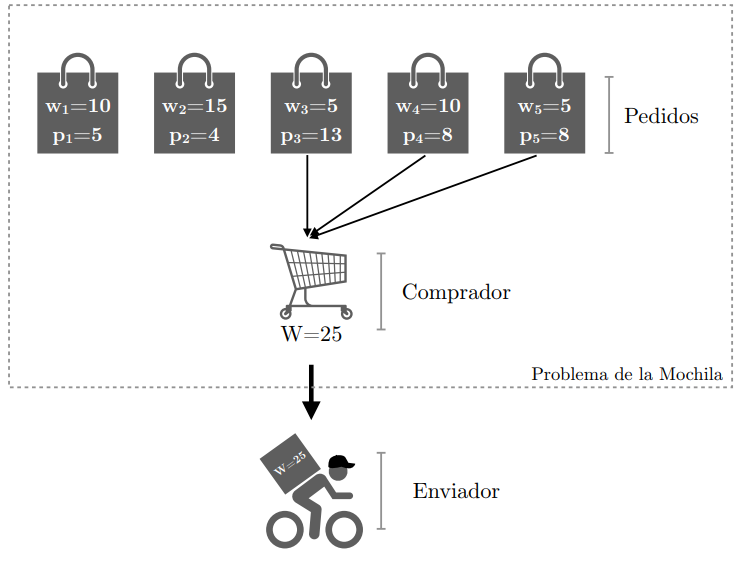
\includegraphics[scale=0.33]{grafiq1.png}
    
    
	\caption{Figura 1.a Caso ejemplo. }
  \end{center}


Para profundizar en la comprensión del Knapsack Problem se puede referir a [1].

\break



\section{Desarrollo}

Para la resolución del problema, elegimos diferentes estrategias algorítmicas. Entendemos que las ventajas y desventajas de cada cual pueden depender del caso a resolver. En primer lugar, presentaremos y analizaremos los distintos algoritmos desde un enfoque teórico. Posteriormente, se experimentará en base a las hipótesis desprendidas de este análisis.  

\subsection{Fuerza Bruta}

\subsubsection{Descripción: ¿Cómo Funciona?}

La primer estrategia utilizada consiste en ir generando todos los subconjuntos de $S$ (el conjunto de pedidos) y, a medida que son generados, ir calculando su beneficio sumando todos los beneficios de sus elementos. Además, se mantiene un registro del tamaño parcial del subconjunto y si en algún momento su tamaño excede a $W$ (capacidad de la mochila), entonces este subconjunto no es válido y se analiza el próximo. Por otro lado, se almacena el valor del mayor beneficio ya calculado y, si el subconjunto actual resulto ser válido, se compara su beneficio con el mayor beneficio ya calculado, el cual se actualiza en caso de ser menor. Una vez analizados todos los subconjuntos, la solución al problema es el mayor beneficio calculado.

A continuación se exhibe el funcionamiento del algoritmo en pseudo-código:

\begin{codesnippet}
\begin{verbatim}

Inicializar result en 0
Para todo subconjunto j de S:
        Calcular beneficio total de j
        result = max( beneficio total de j , result )
Devolver result

\end{verbatim}
\end{codesnippet}

Nótese que en cada iteración del ciclo, result almacena el máximo beneficio de los subconjuntos recorridos.

\subsubsection{Correctitud: ¿Por Qué Funciona?}

Observamos que lo que caracteriza a cada subconjunto y lo distingue del resto es qué elementos de $S$ están incluidos en él y cuáles no. Debido a esto, decidimos representar a los subconjuntos como números naturales de $0$ a $2^n - 1$, donde $n$ es la cantidad de pedidos en $S$; Esto nos sirve ya que el bit menos significativo de la codificación binaria de cada uno de estos números lo interpretamos como ¿Está el primer elemento de $S$?, donde 1 significa sí y 0 no. El segundo bit menos significativo representa al segundo elemento de $S$ y así hasta que el más significativo representa al último elemento de $S$.

Recorriendo desde $0$ a $2^n - 1$ nos aseguramos de recorrer todos los subconjuntos. Como cada elemento tiene la posibilidad de pertenecer o no al subconjunto, es decir dos opciones, la cantidad de casos distintos se puede representar como:

\begin{center}
$ 2_1 * 2_2 * ... * 2_n = 2^n $ (donde n = \#de pedidos)
\end{center}

Con esto vimos que no dejamos casos de lado. Como a todos los subconjuntos les calculamos su beneficio y devolvemos el mayor entre ellos, y como generamos todos los subconjuntos posibles, entonces, el beneficio que devolvemos es el mayor posible.


\subsubsection{Complejidad: ¿Qué Tan Rápido Funciona?}

Para poder determinar la cota temporal de fuerza bruta tenemos que analizar su comportamiento en relación a la entrada:

Recibimos como entrada un vector $S$ de n pares de enteros y un entero $W$.

Analizar cada subconjunto de $S$ cuesta O(n) en peor caso porque para cada bit de su codificación hay que agregar el elemento o no O(1) y tiene a lo sumo n bits, y, por otro lado, son en total $2^n$ subconjuntos.

Basados en esto, hipoteteizamos que la cota teórica temporal de fuerza bruta es $2^n * n$.

\subsection{Meet in the Middle}

\subsubsection{Descripción: ¿Cómo Funciona?}

Meet in the middle es una técnica algorítmica que consiste en dividir la entrada a la mitad, procesar ambas mitades por separado y luego unirlas de alguna forma para obtener el resultado final. Su objetivo es reducir el costo temporal de fuerza bruta sin cambiar drásticamente el enfoque con el cual se encara el problema.

La idea detrás de nuestra implementación de meet in the middle es poder encontrar facilmente el mejor $"$match$"$ de una mitad para cada subconjunto de la otra mitad. Para esto dividimos a $S$ en dos partes a las cuales nos referiremos como izquierda y derecha, donde izquierda es la mitad izquierda de $S$ y derecha la derecha, en caso de que \# de elementos de $S$ sea impar, el elemento extra va a derecha.

Luego, generamos todos los subconjuntos válidos de derecha y los ordenamos priorizando menor tamaño y luego mayor beneficio, esto quiere decir que el menor elemento del vector será aquel cuyo tamaño sea menor y, en caso de empate, cuyo beneficio sea mayor. Por ejemplo, el siguiente sería un vector ordenado correctamente:

\begin{center}
$[$$<0,15>$,$<0,8>$,$<1,17>$$]$
\end{center}

Una vez ordenado de esta manera, lo vamos a recorrer para filtrar los elementos indeseados, es decir, aquellos elementos que no representan un mejor $"$match$"$ para ningún elemento de izquierda. Los elementos restantes son aquellos que representan mayor beneficio para cada tamaño, entonces, nos quedaríamos con los elementos de mayor beneficio de cada tamaño, a menos que exista un elemento de menor tamaño que otorgue mayor beneficio, en ese caso el de mayor tamaño queda descartado. 

Veamos un ejemplo:

\begin{center}
A = $[<0,12>,<1,17>,<1,4>,<2,13>,<2,9>,<4,14>,<5,20>]$

A filtrado = $[<0,12>,<1,17>,<5,20>]$
\end{center}

Lo único que resta ahora es encontrar el mejor match para cada subconjunto de izquierda (generados con el mismo método que en fuerza bruta). Para esto calculamos el $W$ restante restando a $W$ el tamaño del subconjunto de izquierda, y, usando búsqueda binaria sobre tamaño en derecha filtrado, buscamos a $W$ restante para encontrar el mejor match.
Una vez recorrido todo izquierda, devolvemos el mayor beneficio hallado.

\subsubsection{Correctitud: ¿Por Qué Funciona?}

Veamos que dividir a $S$ en dos no nos molesta:

1. Todo subconjunto de $S$ puede ser generado con algún subconjunto de izquierda $\bigcup$ alguno de derecha.

2. Tanto derecha como izquierda contienen al subconjunto vacío (en izquierda puede ser reemplazado únicamente por otro subconjunto de tamaño 0 y que aporte mayor beneficio siendo objetivamente una mejor opción) entonces, dado el caso en que el mejor subconjunto quede todo de un lado, este siempre puede $"$matchear$"$  con vacío.

3. Cuando generamos derecha evitamos agregar subconjuntos que excedan $W$ por ende inválidos e inexistentes en una respuesta correcta. Luego, en el sort solo reacomodamos, no eliminamos ningún subconjunto. Y cuando filtramos nos quedamos con las opciones objetivamente mejores, para cada tamaño el mejor beneficio y suponiendo tamaño p $<$ tamaño r y mayor beneficio de p $>$ mayor beneficio de r, entonces los tamaños r ya no nos sirven y el mejor de r ocupa su lugar, esto vale porque todo subconjunto de tamaño x que podia matchear con tamaño r puede matchear con tamaño p, ya que si \\ 
p $<$ r y x + r $<=$ W entonces x + p $<$ W y al subconjunto de tamaño x le conviene matchear con el de tamaño p porque su beneficio es mayor que el de tamaño r.

\break

\subsubsection{Complejidad: ¿Qué Tan Rápido Funciona?}

Para plantear una cota temporal estudiemos el comportamiento del algoritmo en relación al tamaño de la entrada.

Tomamos como parámetro un vector de pares $S$ de tamaño $n$ y un entero $W$. 

- Generamos $2^{n/2}$ subconjuntos de $S$ y generar cada uno nos cuesta $log_2$ del número que representa al subconjunto así que como máximo $log_2$($2^{n/2}$) $=$ n/2, luego agregamos cada subconjunto al vector derecha costo amortizado O(1). la complejidad teórica de este paso es entonces O($2^{n/2}*n$).

- Ordenamos derecha cuyo tamaño en peor caso es $2^{n/2}$, esto pasa cuando todo subconjunto tiene tamaño menor o igual a $W$. Ordenar cuesta tamaño de lo ordenado $*$ $log_2$(tamaño de lo ordenado $*$ costo de la comparación), en este caso $2^{n/2} * log(2^{n/2}) * 1$ $=$ $2^{n/2} * n$

- Recorremos todo derecha de tamaño máximo $2^{n/2}$ y comparamos 1 vez cada elemento, en peor caso tenemos que agregar todos a un nuevo vector, entonces este paso nos termina costando O($2^{n/2}$) en peor caso.

- Por último, generamos todos los subconjuntos de izquierda que son otros $2^{n/2}$, decodificar cada uno para buscar su tamaño y beneficio nos cuesta su cantidad de bits, es decir $n/2$ y hacer busqueda binaria de su tamaño en derecha nos cuesta $log_2(2^{n/2})$ $=$ $n/2$, entonces el costo total de este paso es O($2^{n/2}*n$)

Basados en este análisis, generamos la hipótesis de que la complejidad temporal de este algoritmo es $O(2^{n/2}*n$).


\subsection{Backtracking}

\subsubsection{Descripción: ¿Cómo Funciona?}

Para desarrollar este algoritmo, nos basamos en la siguiente función recursiva:


$$
maxBen(i, W, S) =  = \left\{
        \begin{array}{ll}
            0 & \quad i = |S| \\
            maxBen(i+1, W, S) & \quad tam(S[i] > W) \\
            max\{maxBen(i+1, w-tam(S[i]), S) + ben(S[i]), \\
            \hspace{0.9cm} maxBen(i+1, W, S)\}   & \quad si no
        \end{array}
    \right.
$$
donde $i$ es el índice con el que recorremos vector que representa a $S$

Analizando esta función, se puede ver que:

$\bullet$ Si no hay elementos por recorrer, el máximo beneficio es 0.

$\bullet$ Si el tamaño del ítem actual es mayor a la capacidad restante $W$, luego el máximo beneficio es el máximo beneficio que puedo obtener con los elementos siguientes a $S[i]$ (sin agregar a $S[i]$).

$\bullet$ Si no se cumplen esas condiciones, luego el máximo beneficio será el mayor entre el máximo beneficio agregando a S[i] y el máximo beneficio no agregándolo. 

A este funcionamiento básico, se le agrega la siguiente poda por optimalidad: si el beneficio del ítem $S[i]$ es mayor al beneficio de todos los siguientes ítems sumados, luego agrego a $S[i]$, sin explorar la opción de no agregarlo. 


\subsubsection{Correctitud: ¿Por Qué Funciona?}

Veamos ahora que es correcto. Nótese que exploran todos los subconjuntos, excepto los que son podados, y nos quedamos con el de mayor beneficio total (y tamaño total menor o igual a $W$). Ahora sólo queda ver que las podas no eliminan casos de más.

La poda de factibilidad, que está descrita en el segundo ítem de la descripción anterior, descarta todos los subconjuntos cuyo tamaño total excede $W$. Por definición del problema, esos subconjuntos no pueden ser solución.

Analicemos entonces la situación en la que la poda de optimalidad se efectúa, esto es, cuando el beneficio del ítem $S[i]$ es mayor al beneficio de todos los siguientes ítems sumados. Cuando esto sucede, se descartan todos los subconjuntos que contienen a los ítems ya seleccionados pero no a $S[i]$. Esto claramente es correcto, pues cualquier subconjunto de los descartados va a tener beneficio menor o igual a uno que contenga a $S[i]$ (y a los ítems ya seleccionados), y, por lo tanto, no puede ser el de máximo beneficio.


\subsubsection{Complejidad: ¿Qué Tan Rápido Funciona?}

La complejidad temporal de este algoritmo en peor caso es $O(2^n)$. Para demostrarlo, alcanza con ver que en el peor caso, es decir, cuando no se efectúa ninguna poda, el costo $T(n)$ es  $T(n-1)+T(n-1)$ más el costo de realizar la comparación, que es constante. Luego, $T(n) = 2 * T(n-1) + c $.  A su vez, podemos ampliar esta ecuación de siguiente forma:

\quad
\begin{center}
    

$T(n) = 2 * T(n-1) + c $

\hspace{2.2cm}$= 2 * (2 * T(n-2)+c)+c$

\hspace{3cm}$= 2 * (2 * ... * 2* T(1)+c) ... + c)$

\hspace{1.2cm}n veces



\end{center}
\quad

De aquí se infiere que $T(n) = O(2^n)$.    

\subsection{Programación Dinámica}

\subsubsection{Descripción: ¿Cómo Funciona?}

Programación dinámica es un método utilizado para resolver problemas dividiendo a estos en subproblemas más sencillos, resolver estos subproblemas una vez y memorizar sus resultados, de esta manera, la próxima vez que este subproblema se presente, como recordamos su resultado no hará falta calcularlo de nuevo. 

Basados en este enfoque, tomaremos el algoritmo de backtracking y lo modificaremos para permitirle memorizar resultados.

La ventaja que esto nos aporta es que a medida que la ejecución recursiva se va desarrollando, irá almacenando los resultados en un diccionario y la próxima vez que estos sean requeridos ya estarán calculados. Fuera de esto, funciona igual que backtracking cuyo algoritmo fue explicado en la subsección anterior.

En este caso, decidimos usar una matriz $M$ porque acceder a sus elementos es muy eficiente. M es de tamaño $N$ (tamaño de $S$) * $W$ (capacidad total de la mochila). Como numeramos a los elementos de $S$ de 0 a $N - 1$, podemos pensar a la matriz como que en su indexación $i$ sobre $N$, cada $W$ y $M$[$i$][$W$] almacena el beneficio óptimo para los elementos $i$...$N - 1$ con $W$ como capacidad máxima.

$M$ originalmente es incializada en -1's, como todos los beneficios son estrictamente positivos, las posiciones definidas con -1's son consideradas inválidas, de esta manera, antes de calcular cualquier resultado nos fijamos si esta ya en la matriz (como la matriz es de tamaño $W$*$N$, todo beneficio óptimo posible tiene su lugar reservado en la matriz, no puede pasar que alguien mas se lo haya ocupado, porque en ese caso sería el y no haría falta recalcularse y no puede no tener espacio, porque entonces sería resultado de un $W$ inválido o de un $N$ inexistente), si esta, lo devolvemos y si no, lo calculamos y lo definimos en $M$.

\subsubsection{Correctitud: ¿Por Qué Funciona?}

El algoritmo funciona porque sigue el mismo procedimiento que backtracking, el cual ya vimos que funciona.

Además, vale aclarar que almacenar resultados en la matriz no interfiere en la correctitud del resultado, porque solo existe un valor óptimo para ese n y w, no puede cambiar a lo largo de la ejecución y como $M$ es inicializada con $-1's$, no hay caso en que esta tenga basura desde el principio, y una vez definida su definición es la correcta.

\subsubsection{Complejidad: ¿Qué Tan Rápido Funciona?}

Para determinar la complejidad temporal de este algoritmo debemos analizar su comportamiento en relación a su entrada, en este caso, un vector $S$ de pares de enteros y un entero $W$ que representa la capacidad total de la mochila.

Lo primero que hace el algoritmo es construir una matriz de tamaño $N$(longitud de $S$) x $W$ y rellenarla con -1's. Este paso nos cuesta $\Theta$($W$*$N$).

Luego, por cada elemento de la recursión, que a lo sumo son $W$ * $N$ (tamaño de la matriz) hay que calcular su beneficio óptimo, esto es hacer función máximo y comparaciones y definir en la matriz, todo O(1) o, si ya esta definido acceder a la matriz que cuesta O(1) también.

Basados en este análisis construimos la hipótesis de que la cota temporal de nuestro algoritmo de programación dinámica es O($W$*$N$).

Notemos que la complejidad espacial de este algoritmo es también $W$*$N$ ya que debemos mantener la matriz.



\section{Experimentación} 
%\input{enunciado}
A fin de corroborar y profundizar los resultados arrojados por el análisis teórico, confeccionamos distintas hipótesis y experimentamos en base a ellas. 

\subsection{Fuerza Bruta} 
Según lo explicado anteriormente, hipotetizamos que la complejidad temporal en peor caso de este algoritmo es $O(n*2^n)$. Obsérvese que el peor caso es aquel en el cual ningún subconjunto tiene tamaño total mayor a $W$. Si bien el nivel de detalle de la descripción en pseudocódigo dada no permite apreciarlo , queda claro al ver en el código fuente, en la función \textit{iesimoBeneficio}, que ni bien se detecta esta condición, se sale del ciclo anticipadamente. 

Por lo tanto, para poner a prueba esta hipótesis, generamos casos (peores) cuyos items tienen tamaño igual a 0 y $W = 1$. En particular, se generaron instancias incrementando $n$ de 1 a 29, con $W$s y tamaños según lo recién descrito, y beneficios con valores aleatorios entre 0 y 100. Para cada $n$, se generaron 30 instancias distintas, se calculó el tiempo que tarda el algoritmo en ejecutarse con esa entrada, y se promedió el tiempo de las 30 instancias. De esta forma, obtenemos un promedio del desempeño del algoritmo, dejando de lado las particularidades de las entradas particulares, y el ruido generado por cuestiones de scheduling del SO. Para $1 \leq n \leq 10 $, se generaron 10000 instancias, ya que, al ser mucho menor el tiempo de ejecución, la influencia del ruido generado por el SO es mucho mayor. 

En el siguiente gráfico se muestra la correlación entre los resultados de la experimentación y la cota $T(n) = n * 2^n $.

\begin{center}
    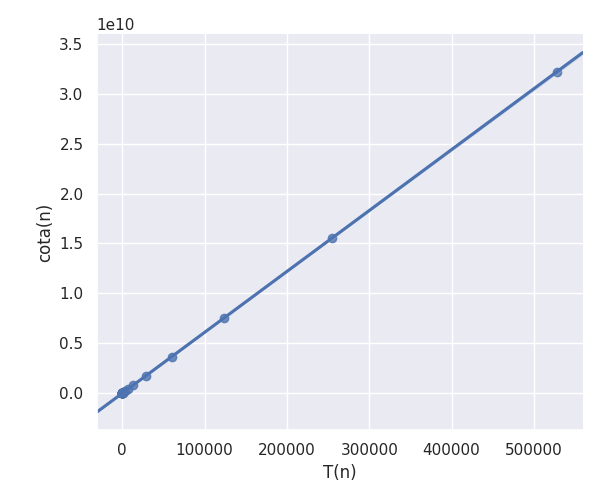
\includegraphics[scale=0.7]{FBcorrelacConCota.png}
    
    
	\caption{Figura 3.1.a  }
  \end{center}

Dado que el coeficiente de Pearson es r=0.9999978520948191, podemos concluir que la hipótesis se corrobora.

Ya respondida esta pregunta, cabe preguntarnos qué pasa con el caso promedio, y cuánto influyen los diferentes parámetros. En particular, sabemos que el beneficio de cada ítem no influye en el flujo de ejecución del programa, excepto por ejecutar una asignación en vez de otra. Así, no consideramos necesario experimentar para corroborarlo. Sin embargo, $W$ y el tamaño de cada ítem sí son valores que influyen en el curso de ejecución, como se explicó recientemente. 

Proponemos realizar un experimento similar al anterior, pero con tamaños aleatorios entre 0 y 50; y $W$ igual a 50, 100, 150 y 200. Como antes, $n$ va a ir de 1 a 29, y nos vamos a quedar con el promedio de 10000 iteraciones, para $n \leq 10$ , y con el promedio de 30 iteraciones para $10 <  n $. Esperamos ver un incremento en el tiempo de ejecución a medida que crece $W$, ya que menos subconjuntos van a descartarse antes de terminar de calcular su beneficio, por exceder $W$ . A continuación se exhiben los resultados:

\begin{center}
    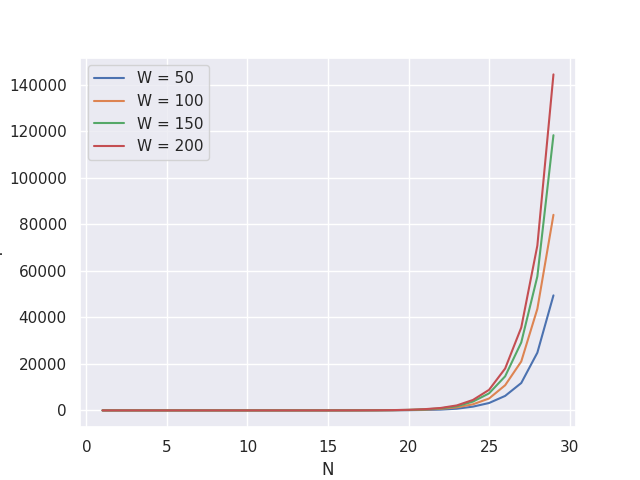
\includegraphics[scale=0.8]{4Quesos.png}
    
    
	\caption{Figura 3.1.b  }
  \end{center}


Puede observarse la clara diferencia entre las distintas ejecuciones. Por ejemplo, obsérvese que para $n = 29$, el tiempo de ejecución con $W = 200$ (144.5 s) casi triplica el tiempo de ejecución con $W = 50$ (49.4 s). Así, concluimos que la hipótesis era acertada.





\subsection{Meet in the Middle}

Por lo visto previamente, nuestra hipótesis de complejidad temporal en peor caso para este algoritmo es $O(2^{n/2}*n$).

Veamos que significa peor caso para esta implementación, generemos en base a esto un caso que lo fuerce y analicemos su relación con la cota teórica.

Podemos ver que el peor caso sucede cuando la mitad derecha de $S$ se mantiene lo más grande posible en todo momento de la ejecución.

Para evitar su reducción entonces, debemos asegurarnos de que el tamaño de ningún subconjunto de derecha de $S$ supere $W$, ya que sino sería inválido y se descartaría. Además, tenemos que evitar que dos de estos subconjuntos pesen lo mismo, y que no haya un subconjunto con mayor beneficio y menor tamaño que otro, esto es para evitar descartar casos al momento de filtrar el vector. Por último, ningún subconjunto de izquierda debe superar $W$, así nos aseguramos realizar el procedimiento de búsqueda binaria con todos.

Dicho esto, nos podemos generar una entrada $S$ en donde todos los elementos de la mitad izquierda posean tamaño 0, evitando así que cuando se conviertan en subconjuntos puedan llegar a pesar más que $W$. Por otro lado, los elementos de la derecha los generamos de manera particular, sabemos que son $n/2$ y que necesitamos que no haya 2 con el mismo tamaño y que todos sean mayor en tamaño y en beneficio que su anterior. Entonces si son $n/2$ elementos, definimos cada uno como $<2^i,2^i>$ para todo $0 <= i < n/2$, de esta manera, al usar potencias de 2 como valores existe una relación directa entre la codificación binaria de subconjuntos que usamos y sus valores. Es decir, el subconjunto 0 es aquel que no incluye ningún elemento, el 1 = 0...01 solo contiene al primero, en este caso $<2^0,2^0> = <1,1>$ el 2 = 0...010 solo al segundo $<2^1,2^1> = <2,2>$, el 3 = 0...011 a la combinación del 1ro y el 2do $<1,1> + <2,2> = <3,3>$, etc. Por último, solo nos falta ver que $W$ tomar para que la suma de ningún subconjunto de derecha lo supere (nótese que todo elemento de izquierda pesa 0), con un razonamiento similar al de recién, vemos claramente que basta tomar $W$ = $i^{n/2}$.

Generamos instancias de peor caso para tamaño de $S$ de 1 a 50, ejecutamos el algoritmo con estas instancias como entrada, y registramos el promedio del tiempo consumido por 10000 iteraciones, para n $\leq$ 10  y por 30 iteraciones, para n $>$ 10. Para ver que tanto se aproximan la cota temporal teórica y la complejidad real en peor caso, realizamos un gráfico de correlación entre estas:

\begin{center}
    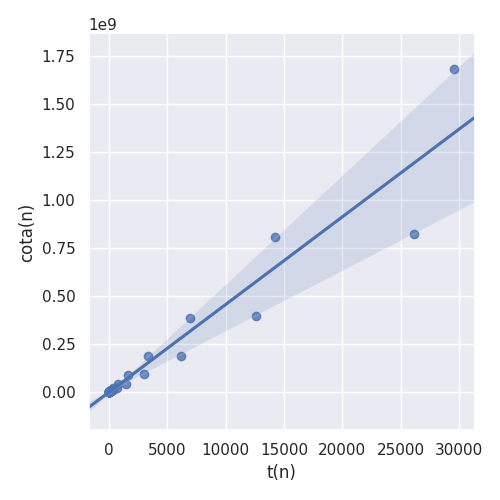
\includegraphics[scale=0.415]{mitmCasoPeor.png}
%	\caption{Figura 3.2.a}
	% _r=0.9595298393150119
	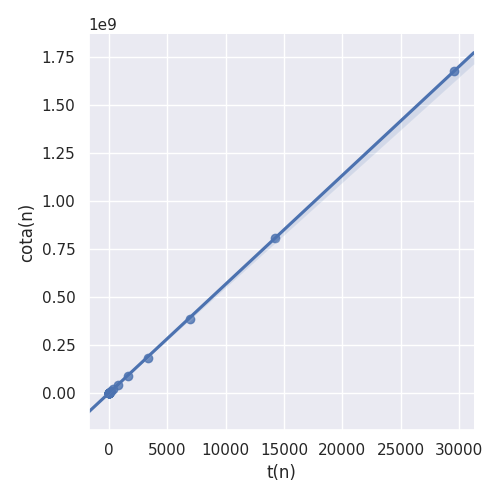
\includegraphics[scale=0.415]{mitmParesPeor.png}
%	\caption{Figura 3.2.b}
	%_r=0.9999852364030486
	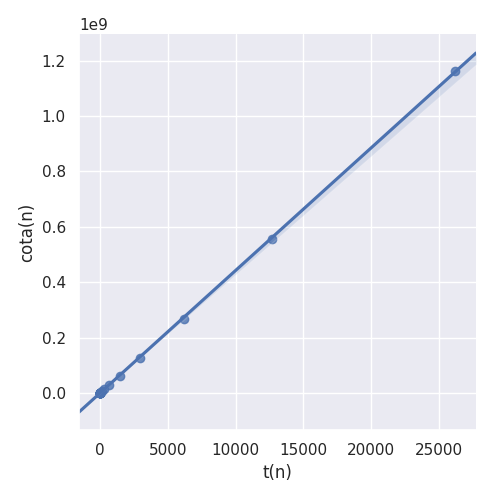
\includegraphics[scale=0.415]{mitmImparesPeor.png}
%	\caption{Figura 3.2.c}
	%_r=0.9999720199203908
	Figura 3.2.a (Todos)   \quad\quad\quad\quad\quad\quad   Figura 3.2.b (Pares) \quad\quad\quad\quad\quad Figura 3.2.c (Impares)
\end{center}

Figura 3.2.a es la imagen que representa el experimento recién realizado, aunque no está tan mal, coeficiente de Pearson = 0.9595, claramente no es lo que esperabamos, podemos ver como esta escalonado a través de la cota. Observamos que esto se produce porque para todo par x y su impar x+1 relacionado, la parte de la cota $2^{n/2}$ da lo mismo, esto no representa precisamente al experimento propuesto.

Para solucionar este problema y ver que la cota de complejidad propuesta originalmente es válida, decidimos analizar los elementos pares y los impares por separado usando exactamente la misma muestra generada en el experimento anterior, de esta forma, logramos analizar el crecimiento de cantidades pares e impares de elementos y compararlos con la cota temporal por separado . Estos nuevos experimentos son los reflejados en Figura 3.2.b (Pares) y en Figura 3.2.c (Impares), y como podemos ver, su correlación con la cota es mucho mas notoria ahora. Ambos exhiben un coeficiente de Pearson = 0.9999 corroborando, o al menos no refutando nuestra hipótesis original.

\break

Para profundizar sobre el rendimiento de este algoritmo, decidimos generar otro experimento,

\begin{minipage}{0.5\textwidth}
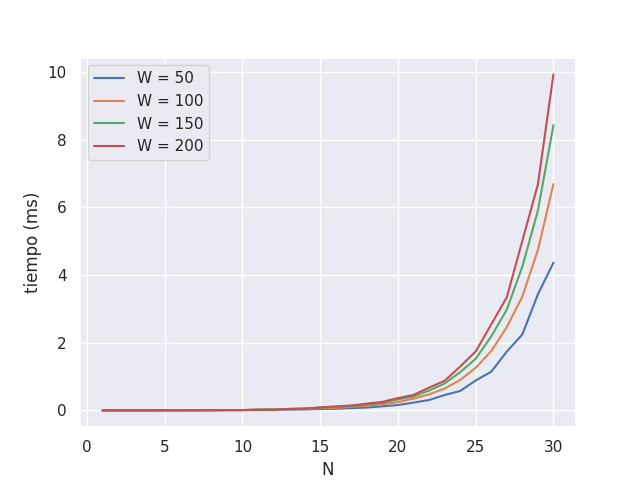
\includegraphics[scale=0.5]{mitmCasoProm4Ws.png}
\end{minipage} \hfill
\begin{minipage}{0.5\textwidth}

En este, queremos analizar el impacto generado por $W's$ de distintos tamaños en el rendimiento del algoritmo, mientras que los tamaños de los elementos de $S$ están acotados siempre por el mismo valor, nuestra hipótesis original es que a medida que $W$ incrementa, también lo hace el tiempo de ejecución. Esto pasa porque si $W$ es menor, entonces en promedio va a costar menos excederlo sumando tamaño de elementos y entonces más subconjuntos serían inválidos y la ejecución se ahorraría ordenar algunos elementos y luego recorrerlos en derecha y hacer búsqueda binaria para algunos de izquierda.

\end{minipage}

Para generar la muestra usada en este experimento usamos la semilla 8 de random de la biblioteca estándar de c++, fijamos $W$ en 50, 100, 150 y 200 para cada caso y todos los beneficios y tamaños de los elementos de $S$ estan dados por un número random módulo 50. El tamaño de $S$, n, lo variamos de 1 a 30, para los N's de 1 a 10 hicimos y promediamos 10000 ejecuciones y para los N's de 11 a 30, 100.

Como podemos ver en el gráfico, a medida que N incrementa la diferencia entre el rendimiento de los distintos $W's$ aumenta, para N = 30, podemos apreciar que la ejecución de $W$ = 200 tarda más del doble que aquella de $W$ = 50. Por otro lado, podemos observar como se respeta nuestra hipótesis ya que la ejecución para $W's$ mayores siempre es más costosa que para $W's$ menores.

Concluimos entonces que nuestra hipótesis no estaba errada.



\subsection{Backtracking}

Como se mostró anteriormente, nuestra hipótesis es que la complejidad temporal en peor caso del algoritmo de Backtracking planteado es $O(2^n)$. Nótese que el peor caso es aquel que resiste a todas las podas. Es decir, aquel cuyos subconjuntos tienen tamaño total menor a $W$, para pasar la poda de factibilidad; y en el cual el beneficio de cada ítem es menor o igual al beneficio total de cualquier subconjunto (excepto el vacío), para pasar la poda de optimalidad. Para generar casos peores, construimos instancias con $W = 1$ y el tamaño de cada ítem igual a 0 (para cumplir la primer propiedad), y el beneficio de cada ítem igual a 1 (para cumplir la segunda propiedad). 

Generamos instancias de peor caso para $n$ de 1 a 30, ejecutamos el algoritmo con estas instancias como entrada, y registramos el promedio del tiempo consumido por 10000 iteraciones, para $n \leq 10$; y por 30 iteraciones, para $n > 10$. Realizamos un gráfico de la correlación entre este tiempo $T(n)$ y la cota de complejidad $cota(n) = 2^n $: 

\begin{center}
    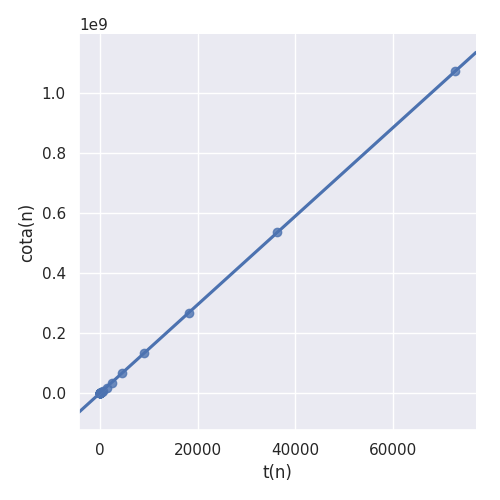
\includegraphics[scale=0.6]{BTcorrelacConCota.png}
    
    
	\caption{Figura 3.3.a  }
  \end{center}

Puede observarse la fuerte linealidad de la correlación, que queda confirmada por un coeficiente de Pearson r=0.9999926249232254. Concluimos entonces que efectivamente  $T(n) = O(2^n)$. 

Para profundizar en la comprensión del rendimiento de este algoritmo, es necesario entender cómo el mismo varía según la entrada provista. En particular, quisimos entender cómo el rendimiento es afectado por los valores dados al beneficio de los ítems. Obsérvese que estos valores afectan el rendimiento sólo por la poda de optimalidad. Analizándolo en detalle, se puede apreciar que los casos que minimizan el tiempo de ejecución deberían ser aquellos con una distribución polarizada, es decir que hay algunos elementos con un beneficio muy grande, otros con un beneficio muy chico, y casi ninguno con beneficio intermedio. De esta forma, es más probable que se dé la situación de poda, es decir, que un ítem tiene beneficio mayor al beneficio total de un subconjunto (en particular, del subconjunto de ítems que no lo contienen a él ni a los ítems ya procesados). Por el contrario, un caso con una distribución concentrada, es decir que hay muchos ítems con beneficio intermedio, y muy pocos con beneficio grande o chico, causaría que la poda se efectúe menos veces, resultando en un tiempo de ejecución mayor. Sería un caso extremo de este efecto, aquel en el cual todos los ítems tienen el mismo beneficio, de forma que nunca se efectuaría la poda 
ya que 
\skip
\begin{center}
    $(\forall{i})(\forall{j}> 0)  w_i \leq \sum_{k = 0}^{j} w_k = j * w_i $
\end{center}

\skip

Para poner a prueba esta hipótesis, y para ver la magnitud de la mejora que aporta la poda de optimalidad, procedimos al siguiente experimento. Generamos 30 instancias de casos con distribución concentrada, es decir generamos sus beneficios de forma aleatoria según una Normal(50,5); y 30 con distribución polarizada, es decir, también generamos sus beneficios según una Normal(50,5), pero luego les sumamos 50 y nos quedamos con el residuo módulo 100 (ver figura 3.3.b y 3.3.c). Para asegurarnos que los beneficios nos den entre 0 y 100, repetimos la generación hasta que así sea. Siguiendo este procedimiento, generamos instancias con $n$ de 1 a 30, y, para aislar el ruido que podría provocar la poda de factibilidad, fijamos $W$ en 1 y los tamaños de los ítems en 0. Ejecutamos el algoritmo con estas instancias como entrada, y registramos el promedio del tiempo consumido por 10000 iteraciones, para $n \leq 10$; y por 30 iteraciones, para $n > 10$. Esperamos ver que las instancias con una distribución concentrada requieren más tiempo que aquellas con una distrubución polarizada.


\begin{center}
  \centering
  \begin{minipage}[b]{0.4\textwidth}
    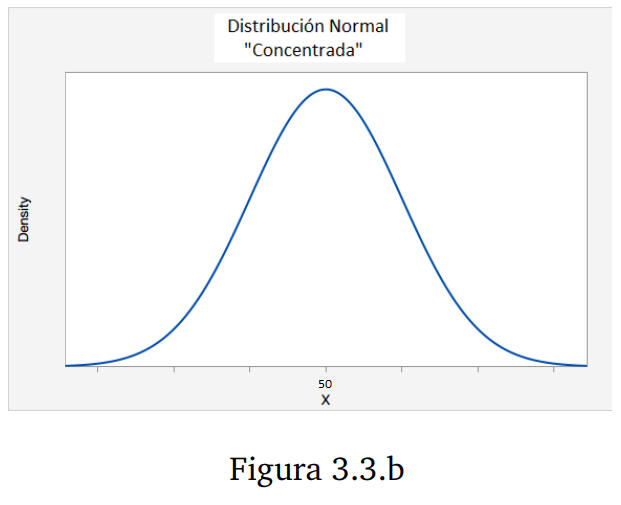
\includegraphics[width=\textwidth]{Concentrada2.png}
    
  \end{minipage}
  \hfill
  \begin{minipage}[b]{0.4\textwidth}
    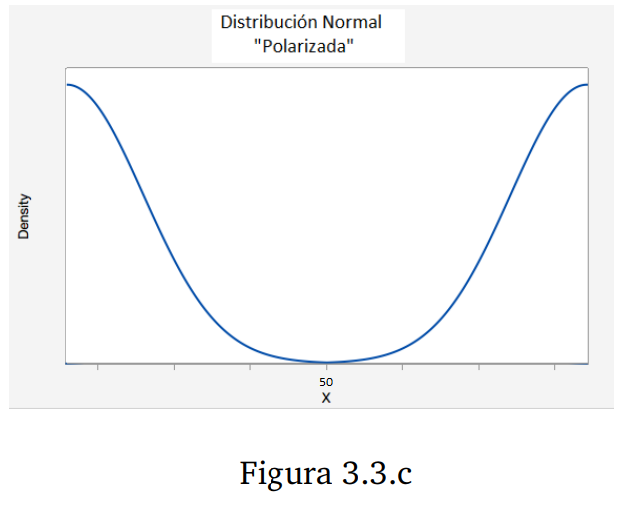
\includegraphics[width=\textwidth]{Polarizada2.png}
   
  \end{minipage}
\end{center}

A continuación se exhibe la diferencia entre los tiempos obtenidos para la distribución concentrada y los de la distribución polarizada, expresada como porcentaje sobre el tiempo de la distribución concentrada. 


\begin{center}
    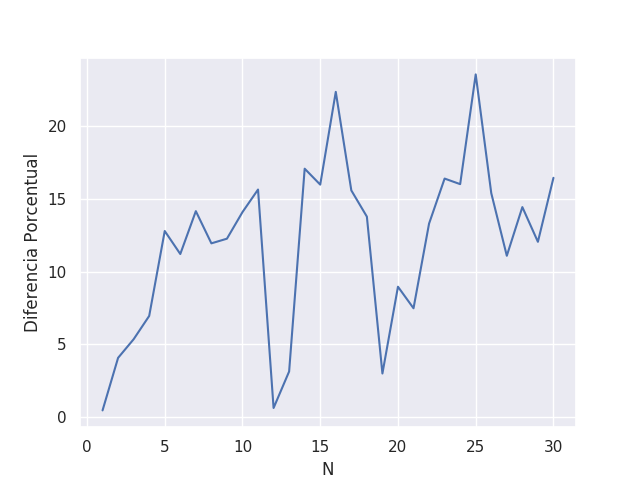
\includegraphics[scale=0.8]{diferenciaPorcentual.png}
    
    
	\caption{Figura 3.3.d  }
  \end{center}

¿Qué se desprende de este resultado? En primer lugar que, como esperábamos, la diferencia es siempre positiva, es decir, los tiempos de ejecución son menores para la distribución polarizada. En segundo lugar, podemos ver que la diferencia alcanza valores mayores al 
$\%20$, lo cual nos sugiere que esta diferencia no es menor. En tercer lugar, el gráfico parece exhibir una tendencia a crecer en función de $n$. Esta última observación no es precisa, se requeriría más experimentación, con mayores $n$s, para descubrir efectivamente esta relación. 

Así, podemos concluir que nuestra hipótesis es corroborada, el algoritmo de Backtracking funciona de forma más eficiente para casos con una distribución de los beneficios polarizada. Las medidas a tomar a partir de estos resultados dependerán de la distribución de los beneficios de los ítems en los supermercados con los cuales se vaya a trabajar en conjunto. 


\subsection{Programación Dinámica}

Como vimos anteriormente, el análisis teórico afirma que la complejidad temporal de este algoritmo es $O(n*W)$, en peor caso. De forma análoga a lo que vimos para Bactracking, el peor caso es aquel que pasa todas las podas. En este caso, es aquel cuyos subconjuntos tienen tamaño total menor a $W$. Para generar estos casos, basta con fijar el tamaño de cada ítem en 0.

Para poner a prueba este resultado, generamos instancias de peor caso con $n$ de 1 a 500, incrementando de a 1, para $n \leq 10 $, e incrementando de a 5, para $n > 10$; el beneficio de cada ítem con un valor aleatorio entre 0 y 100; y $W$ de 1 a 1200, incrementando de a 20. Ejecutamos el algoritmo con estas instancias como entrada, y registramos el promedio del tiempo consumido por 10000 iteraciones, para $n \leq 10$; y por 100 iteraciones, para $n > 10$. A continuación exponemos un gráfico de la correlación entre este tiempo $T(n)$ y la cota de complejidad $cota(n) = n*W $. Nótese que el buen rendimiento de este algoritmo nos permitió realizar experimentaciones cuantitativamente más exhaustivas.  


\begin{center}
    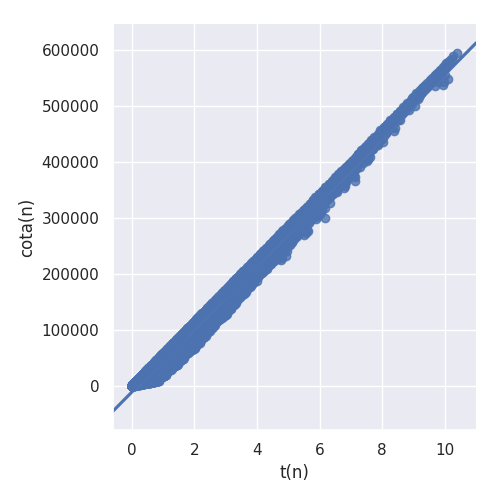
\includegraphics[scale=0.8]{PDcorrelacConCota.png}
    
    
	\caption{Figura 3.4.a  }
  \end{center}

Puede observarse la fuerte correlación lineal, que se confirma por un coeficiente de Pearson r=0.995900081271966. De esta forma, podemos afirmar que efectivamente la complejidad temporal de este algoritmo es $O(n*W)$. 


\subsection{Comparación entre algoritmos}

Hasta ahora hemos analizado la eficiencia de cada algoritmo en función de sus distintos parámetros. Ahora, nos proponemos analizar los distintos algoritmos con un enfoque comparativo que nos acerque aún más a comprender, para cada entrada, cuál algoritmo presenta un mejor desempeño. 

Sin un análisis profundo, en base a los resultados teóricos y experimentales, une se arriesgaría a pronosticar que el algoritmo de Programación Dinámica tarda menos tiempo que los demás para todas las entradas. Sin embargo, una mirada más detenida podría preguntarse si ese es el caso. En particular, el hecho de que la cota de complejidad de PD, a diferencia de todas las demás, depende de $W$, nos hace preguntarnos qué pasa cuando $W$ es muy alta y $n$ muy bajo. Los algoritmos de Backtracking, Meet in the Middle e incluso Fuerza Bruta, dependen "muy poco" de $W$ y "mucho" de $n$, por lo que tendrían tiempos de ejecución bajos. Mientras tanto, PD va a crear una matriz de $nxW$, lo que puede causar tiempos de ejecución más altos. Sin embargo, como la complejidad de PD es lineal en $n$ y en $W$, mientras que las del resto son exponenciales en $n$, esta eventual ventaja se dará con $n$s bajos, hasta que los tiempos de ejecución de los otros algoritmos despunten. 

Para poner a prueba estas hipótesis y encontrar la magnitud en la que se dan estos fenómenos, decidimos hacer la siguiente experimentación. Generamos instancias con  $W$ igual a  150, 1000 y 10000; $n$ de 1 a 28 para Fuerza Bruta, y de 1 a 30 para el resto (excepto para $W = 150$, en cuyo caso $n$ llega a 46); beneficios aleatorios entre 1 y 100; y tamaños aleatorios entre 1 y 50. Ejecutamos los distintos algoritmos utilizando estas instancias como entrada, y quedándonos con el promedio del tiempo de ejecución de 10000 iteraciones, para $n \leq 10$, y el promedio de 30 iteraciones, para $n > 10$.
%fb hasta 28, hmmm ya te digo el otro, creo que 40, esto es 150? o 1000? o 10k? AHH CLARO, con cada w hicimos distintos ehhh
%con 150 es 46
%con 50 fue 30 por mala mia
%y con 1000 y 10k 30 tmb
%yfb siempre 28?
%sip

 A continuación se exhiben los resultados para $W = 150$ y para $W = 10000$.

\begin{center}
	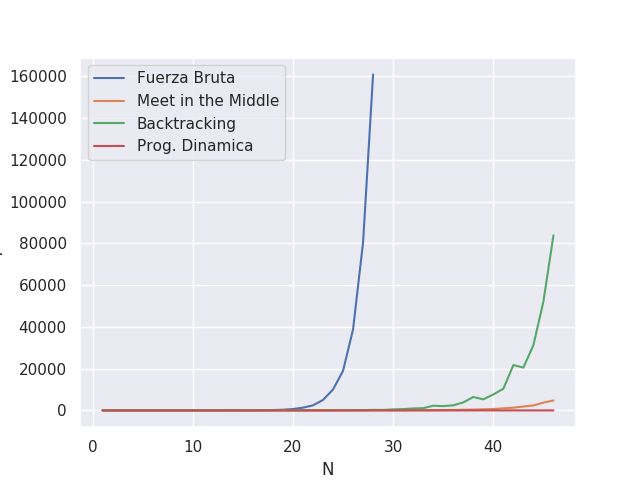
\includegraphics[scale=0.415]{todos150.png}
	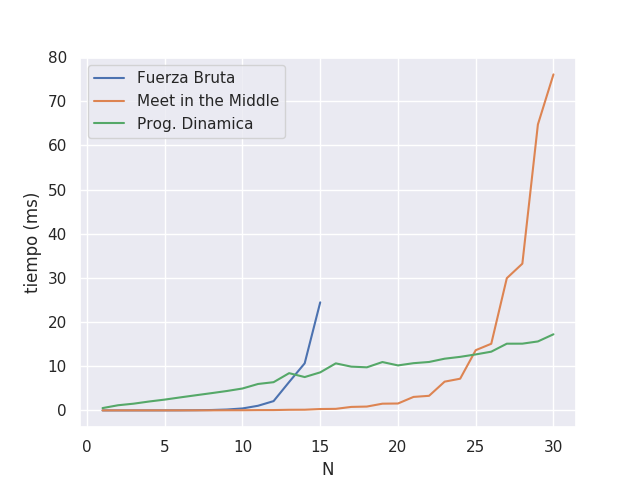
\includegraphics[scale=0.415]{10kfbYmitmVspd.png}
\end{center}

El gráfico confirma que para $W$ pequeño, PD tiene los mejores tiempos de ejecución. Pero, a medida que $W$ crece, esto no es cierto para el caso de los $n$s pequeños. Esta tendencia se empieza a distinguir con $W=1000$, y se aprecia más claramente con $W=10000$. En este último, los tiempos de Meet In The Middle son mejores que los de PD incluso hasta $n = 25$. También FB es más eficiente que PD hasta $n=13$. Estas experimentaciones confirman nuestros pronósticos. Sin embargo, cabe cuestionarse la relevancia de estos resultados: ¿qué valores tomarán $W$ y $n$ una vez comercializado el producto? ¿Se dará el caso de $W=1000$ y $n=25$? Esto dependerá, en parte, de la unidad de medida que se escogerá para $W$, entre otros factores ajenos a nuestro campo de incumbencias.   






\section{Conclusiones}

A lo largo de este informe, se analizaron distintas estrategias para resolver el problema de la mochila, se dedujo su complejidad temporal, se evaluó su rendimiento en función de los valores de sus entradas y se las comparó entre ellas. El algoritmo de Programación Dinámica mostró tener una alta eficiencia temporal. Sin embargo, para $W$ elevadas y $n$ pequeñas, Meet in the Middle resultó más veloz. Por otro lado, la complejidad espacial de PD ( $O(n*W)$ ) es un factor a tener en cuenta. El algoritmo de Backtracking, a su vez, se probó más eficiente para casos cuyos beneficios tengan una distribución más polarizada. Finalmente, Fuerza Bruta obtuvo tiempos de ejecución mayores al resto de los algoritmos. 

Queda pendiente analizar la distribución de los parámetros en las situaciones en las que efectivamente se va a utilizar, para poder así escoger un algoritmo sobre otro. También, se deberá ampliar la solución para poder resolver el Problema de las Mochilas Múltiples. 



\section{Bibliografía}
 [1] Discrete-variable extremum problems. Oper. Res., 5(2):266–288, April 1957.



\end{document}
